\documentclass[8pt,notitlepage,openany]{scrbook}
\usepackage{anysize}
\paperwidth = 13.95cm
\paperheight = 21.6cm
\marginsize{1.5cm}{1.5cm}{0.3cm}{0.3cm} %\marginsize{izq}{der}{sup}{inf }

\usepackage{bera}		% Define el tipo de letra
\usepackage{arev}

%\oddsidemargin = 4cm
%\evensidemargin = 2cm
%\usepackage[left=6.8cm,top=6cm,right=0cm]{geometry} 
%left 0=2.8,
%\documentclass[bsc,draft,singlespacing]{csthesis}
%\documentclass[bsc,doublespacing]{csthesis}
      
\usepackage[spanish]{babel}     % Idioma de Capítulos y demás
\usepackage[T1]{fontenc} 
\usepackage[utf8x]{inputenc}


\usepackage{verbatim}
\usepackage{moreverb}
\let\verbatiminput=\verbatimtabinput
\def\verbatimtabsize{8} 
\usepackage{hyperref}


\usepackage{multicol}

\usepackage{mathcomp}
\usepackage{latexsym}
\usepackage{pifont}
\usepackage{amsfonts}
\usepackage{amssymb}
\usepackage{wasysym}
\usepackage{colortbl}
\usepackage{multicol} 
\usepackage{booktabs}


\usepackage{graphicx}


\setlength{\parindent}{0cm}
\setlength{\parskip}{0.3cm}



\begin{document}
\pagestyle{empty}

%\begin{center}
\hspace{-0.6cm}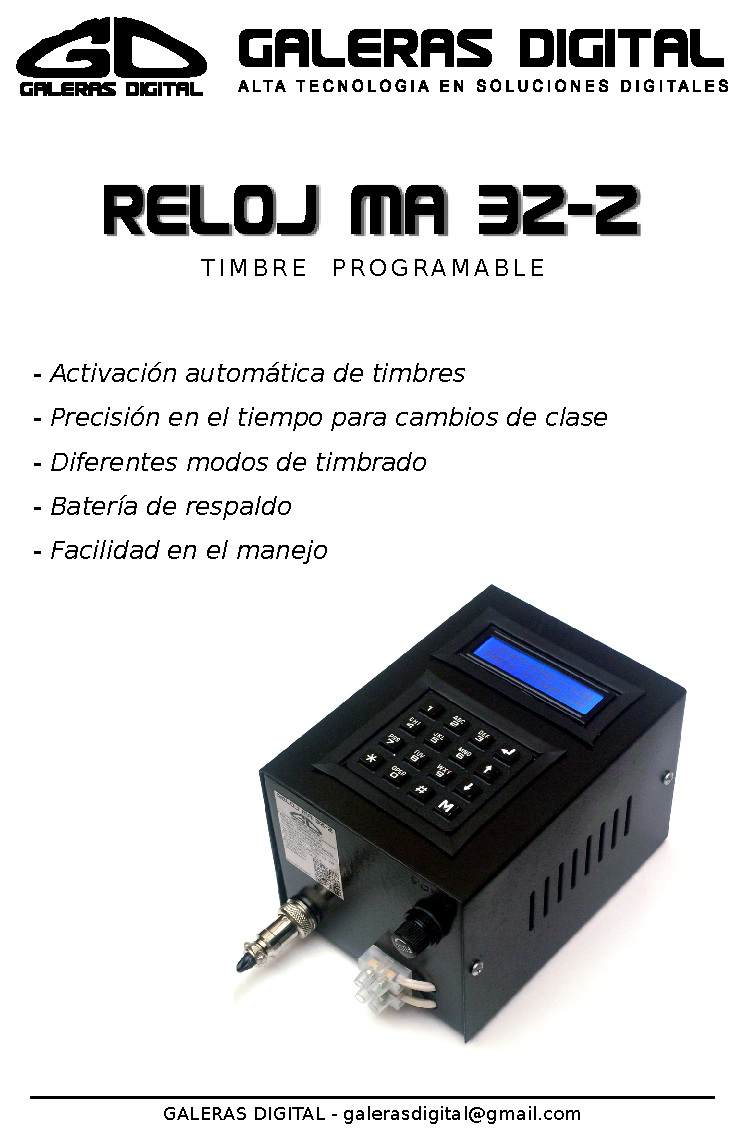
\includegraphics[width=12cm]{partes/tapa.eps}
 % tapa.eps: 1307x2072 pixel, 300dpi, 11.07x17.54 cm, bb=0 0 314 497
%\end{center}


La empresa \textbf{GALERAS DIGITAL}, pone a su disposición el Reloj Multi Alarma MA 32-2.

El Reloj Multi Alarma MA 32-2 es un dispositivo electrónico de alta calidad y precisión que tiene como función principal la activación o ejecución de un timbre, chicharra, alarma u otro equipo similar, de acuerdo a un horario determinado y por un espacio de tiempo programado.

Este equipo fue diseñado especialmente para los establecimientos educativos que marcan el cambio de clase con timbre o chicharra.

\begin{center}
 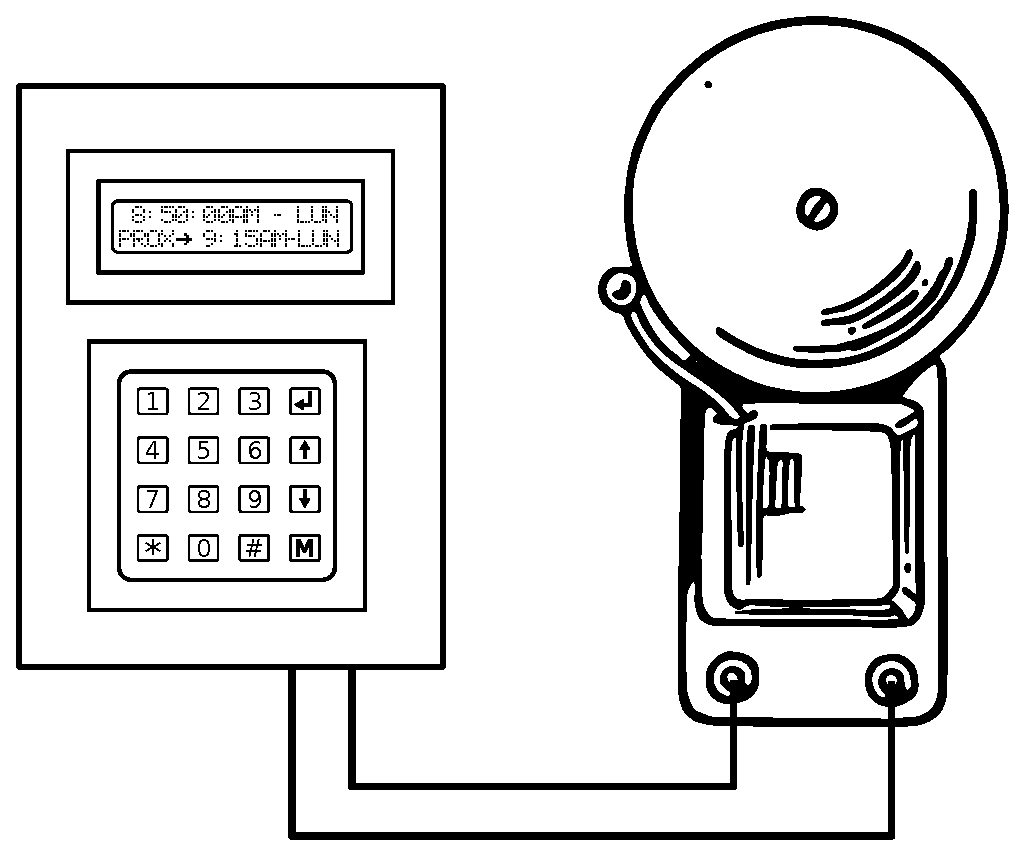
\includegraphics[width=7cm]{partes/timbre.eps}
 % timbre.eps: 824x594 pixel, 300dpi, 6.98x5.03 cm, bb=0 0 198 143
\end{center}


\textbf{Ventajas:}

\begin{itemize}
\item La precisión en el timbre para el cambio de hora, es de gran importancia para toda la comunidad educativa, pero especialmente para el docente quien podrá programar sus actividades de clase con la plena seguridad de que el timbre de cambio de hora sonará con una precisión de segundos.


\item La labor diaria y constante del toque del timbre quedará relegada por completo, ya que el Reloj MA 32-2 se programa sencillamente por una sola vez y no requiere de ninguna otra operación.


\item El funcionario encargado de esta rutinaria tarea quedará libre para dedicar su atención a labores mas productivas para la institución.
\end{itemize}


\textbf{Características:}


\begin{itemize}
\item \textbf{Diferenciación de horarios:} El Reloj MA 32-2 permite programar cuatro horarios distintos  fácilmente intercambiables en diferentes días, cada uno hasta con hasta 30 alarmas.

\item \textbf{Fácil Manejo:} Gracias a su teclado numérico y pantalla LCD, su programación es muy sencilla y se realiza por una sola vez, esta no se borrará aunque se suspenda el fluido eléctrico.

\item \textbf{Pila de respaldo:} El Reloj MA 32-2 cuenta con una pila de respaldo la cual permite al sistema mantener la hora en caso de cortes en el fluido eléctrico. La pila usada, CR2032, tiene una duración de 10 años.

\item \textbf{Seguridad:} El Reloj MA 32-2 posee un sistema de seguridad que solicita una clave o contraseña, para evitar que personas no autorizadas accedan o modifiquen la programación.

\item \textbf{Calidad:} El Reloj MA 32-2 está elaborado con materiales de altísima calidad lo que garantiza un funcionamiento preciso e ininterrumpido durante muchos años.

\item \textbf{Experiencia:} Estos equipos han estado funcionando mas de 3 años consecutivos en las principales instituciones educativas de la ciudad de Pasto, tales como: 

\begin{multicols}{2}

\vspace{-0.2cm}\subitem - Colegio Ciudad de Pasto 
\vspace{-0.2cm}\subitem - INEM
\vspace{-0.2cm}\subitem - Liceo Central de Nariño
\vspace{-0.2cm}\subitem - Libertad
\vspace{-0.2cm}\subitem - Bethlemitas
\vspace{-0.2cm}\subitem - Normal Superior
\vspace{-0.2cm}\subitem - Heraldo Romero
\vspace{-0.2cm}\subitem - LEMO
\vspace{-0.2cm}\subitem - Britanico
\vspace{-0.2cm}\subitem - SUCRE
\vspace{-0.2cm}\subitem - INSUR
\end{multicols}

\end{itemize}

\vspace{-0.3cm}
\begin{center}
 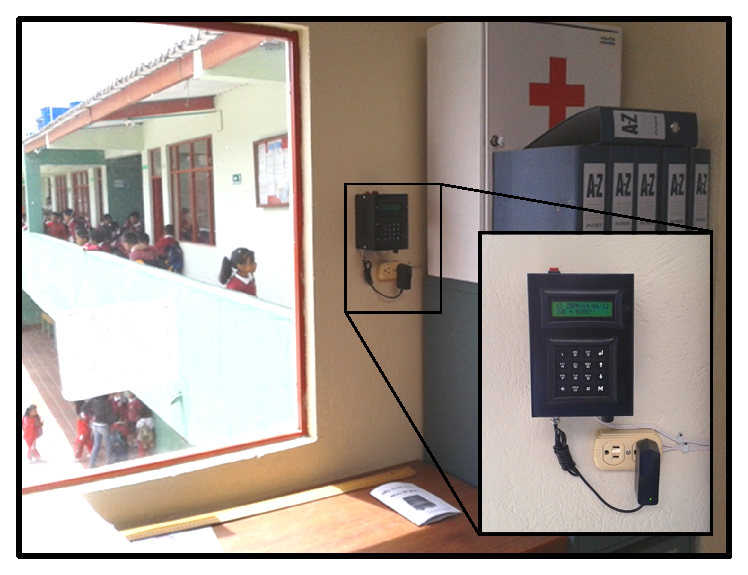
\includegraphics[width=7cm]{partes/fototim.eps}
\end{center}

\begin{small}\begin{tabular}[h]{ll}
\textbf{Costo del Equipo:}&\$545.000 \\
\end{tabular}\end{small}

\vspace{-0.7cm}
\begin{flushright}
\textbf{Garantía por un año}
\end{flushright}

\vspace{0.2cm}

\begin{small}
\textbf{Contactenos:}\\
\\
\textbf{Ventas y soporte técnico:} \\
\hspace*{0.3cm} - Juan Pablo Ruiz: 313 642 8340\\
\hspace*{0.3cm} - Ana Cristina Delgado: 317 260 0591 y 312 764 1311\\
\\
\textbf{Pagina web:} http://www.galerasdigital.com\\
\textbf{Correo electrónico:} galerasdigital@gmail.com\\

\begin{flushright}
\begin{footnotesize}
 GALERAS DIGITAL 2013 \copyright
\end{footnotesize}
\end{flushright}

\end{small}



\newpage
\ \\
\vspace{5cm}
\begin{center}
 
\includegraphics[width=10cm]{partes/tapaf.eps}
 % tapaf.eps: 1111x654 pixel, 300dpi, 9.41x5.54 cm, bb=0 0 267 157
\end{center}
\vspace{3cm}



\end{document}

